\chapter{知识蒸馏~从教师示范到同策略学习}\label{知识蒸馏}

第五章介绍了用奖励或偏好优化模型行为。本章转向另一种训练信号：让学生模型学习教师模型提供的回答或概率分布。知识蒸馏（Knowledge Distillation，KD）把教师的行为迁移给学生，常用于降低部署成本、培养领域能力和传递推理方法。教师可以是更大的通用模型，也可以是某个任务上更强的专家模型。

理解蒸馏可以围绕两个问题：教师提供什么信号，学生在哪些前缀上学习。教师可以提供完整回答，也可以提供下一 token 的概率；训练前缀可以来自教师示范，也可以来自学生当前生成的轨迹。这两个选择共同决定数据构造、损失计算和教师接口的要求。

\section{序列蒸馏~把教师回答变成训练数据}\label{序列蒸馏}

最直接的方式是准备一组问题，让教师生成回答，经检查与筛选后，把问题和教师回答组成 SFT 数据。学生使用教师强制学习目标序列，其训练方法与第四章相同，区别在于目标回答由教师模型提供。只取得文本回答的教师接口就可以支持这条路线，不同分词器的学生可以按自己的词表重新编码回答。

例如，教师为一道方程题生成条件整理、移项与求解步骤，检查器确认结果后，将完整解答交给学生训练。学生学习解题顺序、表达方式和目标答案。收集短答案、完整推导或工具调用轨迹，分别对应不同的行为目标；数据中的长度、难度和任务比例也会影响学生学到的行为。

这条路线通常先生成固定数据，再多轮训练学生，称为离线序列蒸馏。实践中可以为同题生成多个候选，结合执行结果和人工抽查保留高质量示范，再混合原有任务数据训练。训练后分别检查新任务成绩、原有能力与回答成本，选择适合部署的学生版本。

\section{分布蒸馏~学习教师对候选 token 的判断}\label{分布蒸馏}

如果教师接口能够提供下一 token 概率，学生就可以学习整个候选分布。例如，同一个前缀下，教师给三个候选分配 $(0.7,0.2,0.1)$，这份信号既指出首选，也保留了其他续写的相对可能性。对齐这些概率需要教师与学生在同一前缀上预测，并把候选事件对应起来。

一种基础目标是正向 KL：
\[
L_{\mathrm{KD}}(\theta;h)=
D_{\mathrm{KL}}\bigl(\pi_T(\cdot\mid h)\|\pi_\theta(\cdot\mid h)\bigr)
=\sum_{v\in\mathcal V}\pi_T(v\mid h)
\log\frac{\pi_T(v\mid h)}{\pi_\theta(v\mid h)}.
\]
这里，$h$ 是选定的生成前缀，$\pi_T$ 是固定教师的下一 token 分布，$\pi_\theta$ 是参数为 $\theta$ 的学生分布，$\mathcal V$ 是对齐后的共同候选词表，$v$ 遍历候选 token，$\log$ 是自然对数。$L_{\mathrm{KD}}$ 衡量学生与教师在该前缀上的分布差异，训练时再对样本和有效生成位置取平均。优化器更新学生参数，教师保持固定。

直接逐 token 比较时，使用相同分词器与词表最便于对齐；跨词表蒸馏则需要额外构造片段或序列级的对应关系。实际选择还取决于能否获得完整概率、可用带宽和教师前向计算成本。序列蒸馏以教师给出的回答为目标，分布蒸馏则进一步利用候选之间的相对概率。

\textbf{基础阅读}
\begin{enumerate}
    \item Hinton、Vinyals 与 Dean，2015，\href{https://arxiv.org/abs/1503.02531}{Distilling the Knowledge in a Neural Network}。阅读重点：教师概率分布作为训练目标，以及知识迁移与模型压缩的联系。
\end{enumerate}

\section{同策略蒸馏 OPD~让老师反馈学生轨迹}\label{同策略蒸馏 OPD 让老师反馈学生轨迹}

前面的分布蒸馏还需要选择计算反馈的前缀。同策略蒸馏（On-Policy Distillation，OPD）让学生先生成回答，再由教师在学生实际经过的前缀上提供反馈。它把教师指导放到学生自身的生成路径上，可以复用强化学习中的采样和策略更新组件。

模型的错误通常发生在推理轨迹中间某一步。单个最终奖励告诉它``没有做对''，却未必指出从哪个分叉开始偏离；照抄老师的完整解答又主要覆盖老师走过的前缀。我们于是尝试另一种教学安排：学生先自己走，老师在学生走到的位置上给反馈。

OPD 不是 2025 年才突然出现的单一算法，但是直到 2025 年才被广泛关注；广义知识蒸馏（Generalized Knowledge Distillation，GKD）与 MiniLLM 等工作已经研究过相关思路；MiniLLM 是方法名称。不同实现可以使用不同散度、不同轨迹混合与不同梯度估计。我们先理解共同结构，再选一种反向 KL 形式作例子。

在学生生成的前缀 h 上，老师和学生各给出下一 token 分布。反向 KL 把学生分布放在期望的采样侧：学生常选择、老师却不支持的 token，会产生较大的平均代价。若能取得完整分布，就可以对词表求和。 把老师策略记为 π 的下标 T，在同一个学生前缀 h 上，反向 KL 定义为：
\[D_{KL}\left( \pi_{\theta}\|\pi_{T} \mid h \right) = \sum_{v}^{}\pi_{\theta}(v \mid h)\log\frac{\pi_{\theta}(v \mid h)}{\pi_{T}(v \mid h)}\]

求和的 v 遍历词表，θ 表示学生参数；两边必须在同一前缀下给概率。该式是词表分布的 KL，不是单个 token 的人类正确性标签。

若只查询学生实际采样 token 的 log probability，可以用对数概率差构造随机估计，并把相反方向的差作为逐 token 反馈。单个采样差值可以为负，KL 的非负性指的是分布期望；``红色 token''也不自动等于人类语义上确定错误的步骤。 把第 t 步学生前缀记为 h 的下标 t、采样动作记为 a 的下标 t，用老师与学生的对数概率差构造反馈：
\[{\widehat{r}}_{t} = log\pi_{T}\left( a_{t} \mid h_{t} \right) - log\pi_{student}\left( a_{t} \mid h_{t} \right)\]

π 的下标 student 表示用于反馈计算的学生策略，帽号提示这是基于采样的信号。实际实现要说明使用采样时还是更新时的概率，以及哪些量停止梯度。

学生已经走错时，老师面对的是错误前缀。老师可能纠正它，也可能只给出在错误前提下自然的延续。于是，分布反馈很密集，却不等于可靠的步骤真值。通常来说，OPD 方法有效的前提是学生轨迹仍在老师的（正确轨迹）覆盖范围内，允许有一些小偏差。若学生的分布与老师的分布差异过大，则可能收效甚微。

关于正向 KL 散度和反向 KL 散度，我们把两个 KL 方向放回同一幅图景。正向 KL 从老师分布出发，通常更强调覆盖老师的多种模式；反向 KL 从学生分布出发，在受限模型族等条件下常表现出更强的模式选择倾向。本材料讲的相对简略，网络上有许多详细讲解可参考，比如\href{https://zhuanlan.zhihu.com/p/1996277720846471471}{关于正反KL散度}\footnote{https://zhuanlan.zhihu.com/p/1996277720846471471}。

Thinking Machines 在 2025 年的\href{https://thinkingmachines.ai/blog/on-policy-distillation/}{研究博客}\footnote{https://thinkingmachines.ai/blog/on-policy-distillation}中展示了推理与个性化的 OPD 实验，并用采样 token 的老师 log probability 构造密集反馈。低 KL 说明学生接近老师，不能保证接近事实真相；老师的错误、风格偏差与盲点仍会传递。

回到续训退化，我们可以让学生在真实任务前缀上向保留良好行为的老师学习。但老师若没有新课程知识，就不能指望它凭空教会学生。实际还要考虑 tokenizer 对齐、概率接口是否可用、老师计算成本与数据覆盖。OPD 把反馈带到学生路径上，成功条件仍要通过实验确认。

到这里，读者应该自然理解这个教师模型必须与学生模型有完全一样的词表，否则 logits 无法对应训练，也就无法计算 KL 散度，而不同家族的模型词表几乎都是不同的。若老师是黑箱模型，只能给出最终回答，学生就无法在自己的轨迹上逐 token 获得反馈。有了 OPD 也不意味着就可以在任意情况下轻松通过蒸馏把一个弱模型训练成强模型，因为我们首先要有一个同源的强模型，这个强模型通常通过前面的传统方法（SFT 和 RL）训练得到。

那么还有一个问题，如果我们已经有了这个强模型，直接用这个模型不就可以了，为什么还要蒸馏一个小模型呢？原因在于，例如我们要训练一个数学专家模型，准备了一批数学领域的优质 SFT 和 RL 数据，这批数据要与其他领域的许多数据混合以训练一个通用强模型，在这个数据混合的过程中可能存在数据模式冲突，导致类似``1+1<2''的情况出现。但是有了 OPD，我们就不需要关注除了数学以外其他领域的能力，只需要让模型在数学领域成为专家；同样的，其他领域也可以有这种专家模型，然后再通过 OPD 把这些专家模型作为混合教师，蒸馏到一个模型上，这样数据模式冲突的情况就会被规避掉，实践表明这的确收益更高。

\textbf{思考问题}~如果老师是一个黑箱模型，只能给出最终回答，是否还有其他方法实现 OPD？

\textbf{本节相关资料与研究材料}
\begin{enumerate}
    \item Agarwal 等，2023，\href{https://arxiv.org/abs/2306.13649}{On-Policy Distillation of Language Models Learning from Self-Generated Mistakes}，GKD 。阅读重点：学生生成的数据与不同散度目标。
    \item Gu 等，2023，\href{https://arxiv.org/abs/2306.08543}{MiniLLM: On-Policy Distillation of Large Language Models} 。阅读重点：反向 KL 与自回归蒸馏中的优化问题。
    \item Kevin Lu 与 Thinking Machines，2025，\href{https://thinkingmachines.ai/blog/on-policy-distillation/}{https://thinkingmachines.ai/blog/on-policy-distillation/}，\textbf{OPD 最重要的研究博客}。阅读重点：采样 token 反馈的实现与实验条件；它不是普适效率保证。
\end{enumerate}

\section{后训练方法比较 依据信号与分布作选择}\label{后训练方法比较 依据信号与分布作选择}

结合第四章的监督微调、第五章的奖励与偏好优化，以及本章的知识蒸馏，可以按训练信号和轨迹来源选择方法。DPO 使用回答之间的偏好标签，蒸馏使用教师示范或概率反馈；两者分别围绕偏好学习与教师行为迁移组织训练。

我们用三个轴定位：信号从哪里来，轨迹由谁产生并多久更新，优化需要维护什么组件。信号成本也不一定单调下降，老师前向、人工标注与规则验证的价格取决于场景。

\begin{longtable}[]{@{}
  >{\raggedright\arraybackslash}p{(\linewidth - 6\tabcolsep) * \real{0.1567}}
  >{\raggedright\arraybackslash}p{(\linewidth - 6\tabcolsep) * \real{0.2537}}
  >{\raggedright\arraybackslash}p{(\linewidth - 6\tabcolsep) * \real{0.3209}}
  >{\raggedright\arraybackslash}p{(\linewidth - 6\tabcolsep) * \real{0.2687}}@{}}
\toprule\noalign{}
\begin{minipage}[b]{\linewidth}\raggedright
\textbf{方法}
\end{minipage} & \begin{minipage}[b]{\linewidth}\raggedright
\textbf{主要训练信号}
\end{minipage} & \begin{minipage}[b]{\linewidth}\raggedright
\textbf{轨迹或数据来源}
\end{minipage} & \begin{minipage}[b]{\linewidth}\raggedright
\textbf{更新方式}
\end{minipage} \\
\midrule\noalign{}
\endhead
\bottomrule\noalign{}
\endlastfoot
SFT & 目标回答 token & 人类或老师等外部示范 & 最大似然 \\
拒绝采样 RFT & 筛过的成功回答 & 当前或旧检查点采样 & 筛选后最大似然 \\
PPO 类 RL & 结果或过程回报 & 当前或近期策略采样 & 带约束的策略梯度 \\
GRPO 类 RL & 组内相对回报 & 同题多次策略采样 & 相对优势更新 \\
离线 DPO & 被偏好与不被偏好回答 & 固定偏好数据 & 直接偏好损失 \\
OPD & 老师概率或分布 & 学生轨迹或混合轨迹 & 散度或相应梯度估计 \\
\end{longtable}

我们据此决定下一步。若新行为连一条可靠示范都没有，先建设 SFT 示范轨迹数据；若成功路径可采到且可验证，选择 RFT 或者 RLVR 路线；若有明确偏好对但在线训练成本受限，可以选择 DPO 方法；若有现成的强老师模型和可用概率接口，可以考虑 OPD。若问题只是缺少最新课规，回到 RAG，不必先更新权重。

如果读者学完并且基本完全理解了前面的所有内容，那么就已经可以称为是大模型后训练方面的专家了。

\begin{figure}[t]
    \centering
    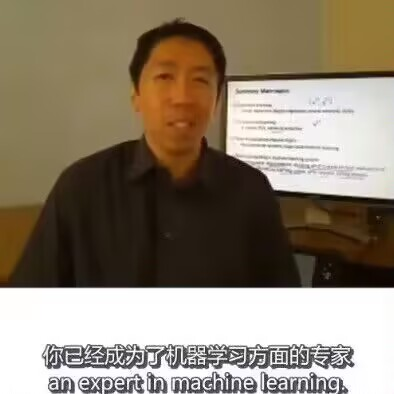
\includegraphics[width=0.7\linewidth]{assets/media/吴恩达-机器学习专家.jpg}
    \caption{你已经成为大模型后训练方面的专家}
\end{figure}